\section{Data analysis \label{sec:data_analysis}}

%MRS: This should be broken up into two sections - 
% The second of which is "what information should be saved - that should really be separated. 
% The first one should be perhaps, " How much simulation data should I collect" and THIS is where we should put discussions of ensembles versus long siulations.  I think the question "how long should I run?" is not the right questions, because as Agastya points out, how to break them up between MULTIPLE runs is an important discussion we should have.

\subsection{How long should I run my simulation for and what information should be saved?}
\label{sec:sim_length_information_kept}
Before launching alchemical free energy calculations it is wise to consider how convergence and completion will be assessed. Different conditions on when to stop alchemical free energy calculations should be determined, and this may require several iterative checks and therefore modifications to the calculation protocol.
One useful metric to use for termination is the expected or desired uncertainty of a desired free energy estimate, though care must be exercised should the uncertainty estimate prove unreliable.
In particular, if the rate of change in the free energy estimate is significant when this condition is met, the simulation may not be locally converged, and more sampling may be necessary to determine a stable free energy estimate which is no longer changing significantly over time. 
A few studies reported systematic variation of simulation lengths using ensemble simulations over an extended range to provide recommendations on appropriate values applicable for most protein-ligand systems. The authors suggest using 4 ns and 10 ns for RBFE~\cite{bhati2017, bhati2022, wan2023eqvsneq} and ABFE~\cite{bhati2025} calculations respectively. These values may be used as a general guideline in cases where the goal is to determine binding affinity for a given starting structure. However, these guidelines do not hold if one is interested in studying the kinetics and/or the starting structure available is not representative of the equilibrium structure.

However, this is not the only metric which can or should be used, as the uncertainty only captures the information about the sampled phase space, not necessarily the entirety of the phase space.  
For example, convergence of relative free energy calculations in predictive simulations where the entire phase space is not known in advance requires sampling the different kinetically stable states~\cite{mobley2012perspective}. 
This highlights the importance of choosing the correct thermodynamic path to ensure you sample the required thermodynamic states as discussed in Sec.~\ref{sec:important_path}.

The condition of minimizing the statistical uncertainty of different free energy estimators below a sufficient threshold should be one metric monitored over the simulation. This can be done through the uncertainty estimator built into certain analysis tools such as MBAR, or through more general statistical tools like bootstrap sampling. It should be noted however, that uncertainty estimates have the same limitations as other metrics of convergence, as they are only an uncertainty based on the phase space sampled so far in a simulation, and cannot account for states not sampled, and it is worth considering that they will be an underestimation of the true uncertainty~\cite{wan2020fep+, wan2021uq, vassaux2021, gapsys2020large, wade2022, bhati2017, bhati2022, bhati2025, wan2023eqvsneq, bhati2018, bhati2019, cournia2017relative, gapsys2021accurate, baumann2021challenges, caves1998locally}.
A target statistical uncertainty should be chosen at the onset of the simulation to avoid excessively long simulations, or falling into the trap of running until the free energy estimate is "good enough," which is subjective and has no defined criteria. This could be a fixed value such as $0.20$ kcal/mol, or a functional quantity such as "below $0.5$ kcal/mol and $10\%$ of the free energy estimate." The user does not need to monitor this information in real-time and can choose to run simulations for fixed duration (either time or number of samples) and run analysis on the data collected thus far. If more samples are needed, the simulations can be resumed, or, started again in different initial conditions enlarging the overall simulation ensemble. 
Bhati et al. recommended such a scheme for RBFE and ABFE calculations using TIES~\cite{bhati2022, bhati2025, wan2023eqvsneq, coveney2022corners}. They suggest a set of optimal parameters (ensemble size, simulation length, number of lambda-states, number and length of NEQ transitions, etc.) to be used initially and suggest pre-defined criteria (uncertainties below 0.5 kcal/mol and overlap between forward and reverse work values in case of NEQ calculations) to decide on the need of additional calculations (in the way suggested) until these criteria are met.

\begin{figure}
    \centering
    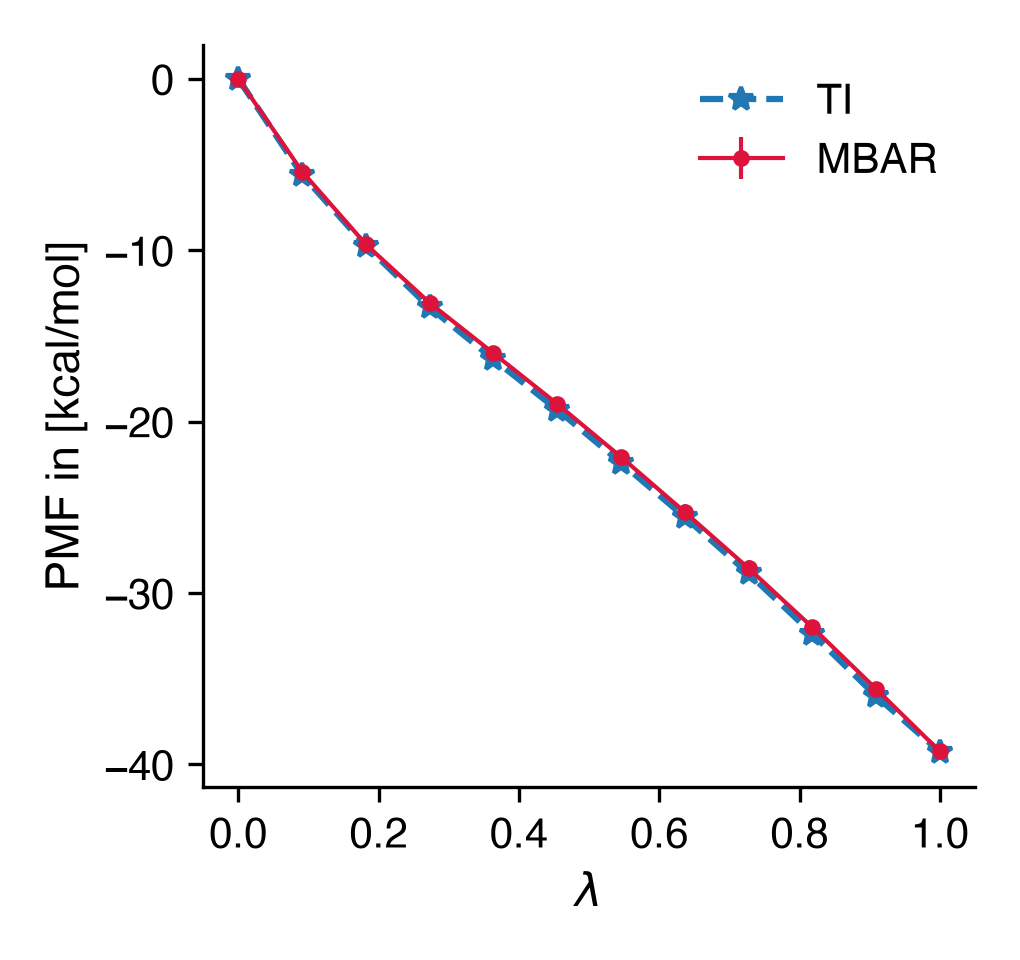
\includegraphics[width=0.8\linewidth]{figures/fig_pmf/pmf.png}
    \caption{{\bf Potential of mean force with respect to $\lambda$ for TI and MBAR}
    The estimated PMF for a bound calculation of a Tyk2 ligand pair of Wang et al.~\cite{wang2015accurate} with respect to $\lambda$ estimated from TI and MBAR and showing agreement within errorbars. 
    }
    \label{fig:pmf}
\end{figure}

The uncertainty in the free energy, for example, can be estimated in multiple ways, e.g. through standard error propagation methods (including MBAR's estimator, which is based on the same principles as standard error propagation), through bootstrap methods, and through ensemble simulations. 
%However, as we have repeatedly pointed out, only ensemble simulations can capture the true uncertainty in MD based predictions. All other methods underestimate the true uncertainty as reported by several authors~\cite{wan2020fep+, wan2021uq, vassaux2021, gapsys2020large, wade2022, bhati2017, bhati2022, bhati2025, wan2023eqvsneq, bhati2018, bhati2019}. 
Independent of how the property is estimated, it is important to remember that results of any free energy analysis are \textit{estimations of the given property}, not the true underlying value of the property itself. 
These estimators are usually consistent estimators, meaning they will converge to the true answer in the limit of sufficient sampling, not necessarily unbiased ones though.
As such, it is a good idea to subject different estimators to the same data to see if they yield either the same estimate (within error and bias), or if they fluctuate wildly. See, for example, the potential of mean force with respect to $\lambda$ estimated from a bound simulation of a Tyk2 ligand pair of Wang et al.~\cite{wang2015accurate} for both the MBAR and TI estimators, as seen in Fig.~\ref{fig:pmf}.
This is not a perfect method as some estimators, such as exponential averaging, will converge significantly more slowly, relative to more accurate estimators like MBAR. 
Therefore, it is a good idea to apply the estimators to different fractions of the data to see if the main estimator of free energy you have chosen is stable.

Each method requires different data from the simulation be collected. If, for instance, the free energy estimator selected is thermodynamic integration, then values of $\frac{dU}{d\lambda}$ at uncorrelated data points must be collected. Once you have made a choice of the combination of the type of simulation you will run, which alchemical topology you will simulate, what alchemical path you will simulate along, and what your stopping conditions are, then you are ready to enumerate the information you should capture. Below is a sample of the minimal information you need for a set of common estimators (discussed in more detail in Sec.~\ref{subsec:estimators}):

\begin{itemize}
    \item Thermodynamic integration (TI) requires $\frac{\partial U(q)}{\partial\lambda}$.
    \item Exponential averaging (EXP) needs \textit{either} $\Delta U_{k,k+1}(q)$ or $\Delta U_{k,k-1}(q)$, depending on the direction its being evaluated in.
    \item Bennett acceptance ratio (BAR) needs \textit{both} $\Delta U_{k,k+1}(q)$ and $\Delta U_{k,k-1}(q)$.
    \item Weighted histogram analysis method (WHAM) and multistate Bennett acceptance ratio (MBAR) both need the complete set of $\Delta U_{k,j} \, \forall \, j=\{1...K\}$. WHAM must have this same information binned with some choice of bin width small enough not to affect the results.
\end{itemize}

The potential derivative required for TI should generally be calculated during the simulation; only under very rare circumstances~\cite{naden2015linear} can it post-processed by a code that does not evaluate the derivatives. Many codes already have options for doing this.
If that option is unavailable, you can estimate it through finite difference (if sufficient information is collected), but this will introduce significant error, and is generally not a best practice. The BAR estimator may be a better, and simpler choice at that point as you will have at least the same level of information. 

The potential energy differences required for EXP, BAR, MBAR, and WHAM can be calculated either during the simulation or in post-processing. It is recommended to calculate the potential differences in code when possible to avoid extra overhead and possible errors produced by evaluating the energy of the configuration twice, and to reduce the amount of stored information. 
Although potential energy derivatives must usually be calculated in code, they can sometimes be easily computed in post-simulation analysis. 
For example, if the alchemical path you have chosen is a linear alchemical path, then $\frac{dU}{d\lambda} = U_1(q) - U_0(q) = u(q)$, which is the perturbation energy $U$--the potential energy difference between the initial and final states. These values are already calculated by the simulation and can be recorded easily without additional computational expense. As discussed earlier, linear paths are inefficient. However, methods such as EDS and ATM, based on optimized non-linear energy interpolation alchemical energy functions $W_\lambda(U)$ that depend on atomic coordinates only through the perturbation function~\cite{konig2021efficient,azimi2022relative}, can achieve high computational efficiency by sampling and storing only perturbation energy values. The stored values can then be analyzed in post-processing to, for example, evaluate algebraically the $\Delta U_{k,j}$ quantities needed by multistate analysis (see above). 

Free energy information should generally be saved more frequently than coordinate data, approximately at the rate that uncorrelated samples are produced.  
The on-disk size of the data for free energy estimation is often significantly smaller than full atomic coordinates, so the information can easily be collected frequently. 
However, the information should not be collected \textit{every} time step, as most free energy techniques are operated at equilibrium, and need equilibrated \textit{and decorrelated} samples for an unbiased estimate.
Samples collected every time step will likely result in most samples being discarded due to the detection of correlation in the time series by decorrelation routines in the analysis. However, if it is computationally cheap and disk space is plentiful, do save often. One may safely assume that the correlation time is greater than 100-200 fs even for relatively simple systems such as small molecules in solvent, so saving no more frequently than every 50-100 steps is recommended. 
How decorrelation impacts calculations, and how to compute it is discussed in Sec.~\ref{sec:subsampling}.

In general, uncertainties can be assumed to decrease as $N^{-\frac{1}{2}}$ where $N$ is the number of uncorrelated samples (not the number of atoms!), for all standard free energy calculation methods~\cite{shirts2005comparison}. However, this carries the notable caveat that such estimates require accurate estimation of the correlation time which, if important motions are slow compared to simulation timescales, can be difficult. Still, this metric provides a good rule of thumb, and as long as conformational transitions are captured by the simulation, increasing the aggregate simulation time by a factor of $T$ will reduce the uncertainty by a factor of approximately $\sqrt{T}$.

Once data has been collected from alchemical intermediates, it must be analyzed to produce an estimate of the free energy change (and its associated statistical uncertainty) for each leg of the thermodynamic cycle.
While a number of different estimators are available that will give consistent results under optimal circumstances, some approaches are recommended over others due to their robustness and ability to provide information on poor convergence.

\subsection{Estimators for free energy differences}
\label{subsec:estimators}
Free energy differences between two different states differing in the energy function are directly related to the
ratio of probabilities of those states.
The partition functions in, for example, Eq.~\ref{eq:DG-solvation-excess}, are simply the total accumulated probabilities for all possible configurations of the system. Virtually all of the ways to estimate this free energy difference are based on converting this ratio of integrals to something that can be measured in simulations.  

\subsubsection{The Zwanzig relationship (EXP)}
The simplest method for calculating free energy differences from simulations is the so-called \textit{Zwanzig
relationship}~\cite{zwanzig1954hightemperature}, also called one-sided exponential re-weighting (EXP), or simply free energy perturbation, though this final term is sometimes used to encompass all ways of calculating free energy differences.

The reduced free energy difference $\Delta f_{01}$ between an initial state 0 and a final state 1 defined by two reduced Hamiltonians $\mathcal{H}_0(q,p)$ and $\mathcal{H}_1(q,p)$, where $\mathcal{H} \equiv \beta H$, can be calculated as:
\begin{eqnarray}
\Delta f_{01}  =  -\ln \expect{e^{- (\mathcal{H}_1(q,p) - \mathcal{H}_0(q,p))}}_0 =  -\ln \expect{e^{- \Delta \mathcal{H}(q,p)} }_0
\end{eqnarray}
and the average is over all samples from the simulation performed with $\mathcal{H}_0$.
The contribution to free energy difference due to the kinetic partition function can be factored out and cancels out in a thermodynamic cycle when calculating double free energy differences, as discussed in Sec~\ref{sec:chemical_potential}.
This allows focusing on configurational partition function and express free energy estimator using the reduced potential energy difference $\Delta u(q)$
\begin{eqnarray}\label{eqn.zwanzig_configurational}
\Delta f_{01}  =   -\ln \expect{e^{- \Delta u(q)} }_0
\end{eqnarray}

Described in words, we take the samples generated during our run with the reduced potential $u_0(q)$ and calculate what the difference in energy would be if we switched instantaneously to the reduced potential $u_1(q)$, and average the exponential of the negative energy difference to get the negative of the exponential of the free energy difference. The original distributions, P($u_0$) as generated at $\lambda=0$ and P($u_1$) would look like those seen in Fig.~\ref{fig:fig_sampling_scheme}\textbf{A}-\textbf{C} on the right hand side. Reevaluating requires almost no extra code functionality to perform; one need only to save a full precision trajectory, and run an unmodified molecular simulation code using the $u_1$ in order to calculate the new energies of stored snapshots. The analysis can be written in a line of code.

Although the Zwanzig equation is formally correct as long as the two states considered sample the same phase space volume, which is true for standard molecular models, it has some very important numerical issues that mean that it often performs badly for standard free energy calculations, even for small molecules~\cite{shirts2005comparison,lu2003appropriate}. One can show that if the standard deviation of the difference $\Delta u(q) = u_1(q)-u_0(q)$ over all sampled $q$ is large, which in this case means more than a few units (equivalent to a standard deviation of only several times $k_BT$ in $\Delta U(q)$), then very few samples contribute to the average, and the answer will be both biased and extremely noisy~\cite{lelievre2010free}. Essentially, the method is dominated by contributions of rare snapshots~\cite{jarzynski2006rare, wu2005phasespace, wu2005phasespacea}. 

 As a reminder, the estimators in this section are written in terms of the reduced potential $u$, reduced free energy $f$ and reduced work $w$ introduced in Sec.~\ref{subsec:numerical-implementations}, which keeps them valid in any ensemble.
 
The Zwanzig formulation is general in that the instantaneous work to change the reduced potential from $u_0$ to $u_1$ can be replaced by the non-reversible reduced work $w$ to make the same change beginning from the same equilibrium conditions at either end state~\cite{jarzynski1997nonequilibrium,jarzynski1998equilibrium,crooks2000pathensemble}, allowing for non-equilibrium free energy calculations, an alternate approach. 
%We do not detail non-equilibrium transformations here, and refer the reader to more advanced treatments~\cite{maragakis2008bayesian,oberhofer2005biased,procacci2015unbiased,shirts2003equilibrium,ytreberg2004singleensemble, gapsys2020large}.

\subsubsection{Jarzynski's Equality}
Jarzynski's equality relates the reduced work ($w \equiv \beta W$) obtained from a one-directional non-equilibrium transition to the free energy difference between the end states:

\begin{eqnarray}\label{eqn.jarzynski}
\langle e^{-w} \rangle =e^{-\Delta f}
\end{eqnarray}

The work of an alchemical transition can be calculated by integrating $\partial \mathcal{H}(q,p)/\partial\lambda$ over the transition path:

\begin{equation}\label{eqn.work_value}
w   = \int_{0}^{1} \frac{\partial \mathcal{H}(q,p)}{\partial\lambda} d\lambda.  
\end{equation}

Expressing $\Delta f$ directly from Jarzynski's equality gives an estimator for the free energy difference, which is equivalent to Zwanzig's estimator when a transition is performed instantaneously:

\begin{eqnarray}\label{eqn.jarzynski_estimator}
\Delta f = -\ln\langle e^{-w} \rangle
\end{eqnarray}

This estimator, however, is biased, and the bias depends strongly on the reduced dissipated work $w_{\mathrm{dis}}=w-\Delta f$~\cite{gore2003bias}.
The bias vanishes only for infinitely slow transitions where $\Delta f = \lim\limits_{\tau \to \infty} w$.
When work distributions are Gaussian, $p(w) \sim \mathcal{N}(\overline{w},\sigma_w^2)$, the Jarzynski estimator becomes:

\begin{eqnarray}\label{eqn.jarzynski_gaussian}
\Delta f = \overline{w} - \frac{\sigma_w^2}{2}
\end{eqnarray}

The assumption of Gaussian work distributions usually holds only for slow switching that keeps the system close to equilibrium~\cite{jarzynski1997nonequilibrium}, so its use should be carefully monitored.

\subsubsection{The Bennett acceptance ratio (BAR)}
If we have the differences in the potential energy sampled from the distribution defined by $u_0$ to the state defined by $u_1$, and we also have the differences in potential energies from the distribution sampled by $u_1$ to the state defined by $u_0$, we can obtain a significantly improved estimate of the
free energy difference compared to that obtained by EXP. 
This estimate was first derived by Bennett and is hence generally called the Bennett Acceptance Ratio (BAR). It is solved by finding the reduced free energy difference $\Delta f$ that satisfies the following implicit equation:

\begin{eqnarray}
 \sum_{k=1}^{n_i} \frac{1}{1 + \exp[\ln(\frac{n_i}{n_j}) + \Delta u_{ij}(q_k) - \Delta f_{ij}
 ]} \nonumber \\
 =\sum_{l=1}^{n_j} \frac{1}{1 + \exp[\ln(\frac{n_j}{n_i}) - \Delta u_{ij}(q_l) + \Delta f_{ij}]}, \label{eq:bar}
\end{eqnarray}

where $n_i$ and $n_j$ are the number of samples from each state. More recent derivations show that this formula is the maximum likelihood estimate of the free energy difference given sets of samples from the two states~\cite{shirts2003equilibrium}. 
The equation does not have an explicit solution for $\Delta f$ and needs to be solved numerically to obtain the estimate for free energy difference.

Many studies have demonstrated both the theoretical and practical superiority of BAR over EXP in molecular
simulations~\cite{shirts2005comparison,lu2003appropriate}, and BAR converges to EXP in the limit that all samples are from a single state~\cite{bennett1976efficient,bennett1976efficient,shirts2003equilibrium}. BAR also requires significantly less overlap between the configurational space of each state to converge than EXP, though some overlap must still exist.

The Bennett acceptance ratio is only defined between two states. Usually, the endpoints of interest in a free energy calculation are sufficiently different that we will need a chain of states that gradually change the reduced potential from $u_0$ to $u_1$, as discussed in Sec.~\ref{sec:important_path}. You can carry out a BAR estimate between each pair of states $\Delta f_{1 \rightarrow N} = \Delta {f_{1\rightarrow 2}} + \Delta {f_{2\rightarrow 3}} +  \ldots + \Delta f_{N-1\rightarrow N}$.

There is one important thing to note about the uncertainty estimates when summing multiple free energy differences together to calculate an overall estimate of a free energy difference. Although BAR itself gives a free energy estimate that is asymptotically correct and is much less biased than the uncertainty estimate for EXP, the uncertainties in $\Delta {f_{i-1\rightarrow i}}$ and $\Delta {f_{i\rightarrow i+1}}$ are not uncorrelated, because they both involve the energies $u_i(q)$. The variances of each of the free energies cannot simply be summed together into the variance of the overall free energy. Instead, some other method for propagating the uncertainty, such as bootstrapping~\cite{grossfield2018best} must be used.

\subsubsection{Bennett Acceptance Ratio for non-equilibrium transitions}
Similarly to the analogy between Zwanzig's and Jarzynski's equations, Bennett Acceptance Ratio can be applied to estimate free energy differences from non-equilibrium transitions as well.
Replacing $\Delta u_{ij}(q)$ in equation~\ref{eq:bar} by reduced work values $w_k$ and $w_l$ corresponding to the work observed for the forward and reverse transitions, BAR can be written as follows~\cite{shirts2003equilibrium}:

\begin{eqnarray}
 \sum_{k=1}^{n_F} \frac{1}{1 + \exp[\ln(\frac{n_F}{n_R}) + w_{k} - \Delta f]} \nonumber \\
 =\sum_{l=1}^{n_R} \frac{1}{1 + \exp[\ln(\frac{n_R}{n_F}) - w_{l} + \Delta f]}, \label{eq:bar_noneq}
\end{eqnarray}

Another approach to estimate free energy from bi-directional transitions relies on the Gaussian approximation of work distributions similarly as described earlier for uni-directional transitions (eq.~\ref{eqn.jarzynski_gaussian})
When work distributions for the forward and reverse transitions can be approximated by Gaussians $\mathcal{N}(\overline{w_f},\sigma_f)$ and $\mathcal{N}(-\overline{w_r},\sigma_r)$, respectively, the free energy difference between the states is defined as an intersection point between the distributions, hence, termed Crooks Gaussian Intersection (CGI)~\cite{goette2009accuracy}:

\begin{eqnarray}\label{eq:cgi_noneq}
 \Delta f = \frac{\frac{w_f}{\sigma_f^2}-\frac{-w_r}{\sigma_r^2}\pm\sqrt{\frac{1}{\sigma_f\sigma_r}(w_f+w_r)^2+2(\frac{1}{\sigma_f^2}-\frac{1}{\sigma_r^2})\ln{\frac{\sigma_r}{\sigma_f}}}}{\frac{1}{\sigma_f^2}-\frac{1}{\sigma_r^2}}
\end{eqnarray}

The estimate above holds for distributions where $\sigma_f \neq \sigma_r$.
For the case of $\sigma_f=\sigma_r$, free energy difference is estimated as $\Delta f = (w_f-w_r)/2$.

\subsubsection{Thermodynamic integration (TI)}
By taking the derivative of the free energy with respect to the
variable $\lambda$, we find that:
\begin{equation}
\frac{df}{d\lambda} = \frac{d}{d\lambda} \left[-\ln \int \frac{\exp^{-u(\lambda,q)}}{Z(\lambda)} dq\right] = \expect{\frac{du(\lambda,q)}{d\lambda}\
}_{\lambda} .
\end{equation}
And then we can numerically integrate $df/d\lambda$ over an alchemical transformation, using a range of different well-established techniques, to obtain:
\begin{equation}
\Delta f    = \int_{0}^{1} \expect{\frac{du(\lambda,q)}{d\lambda}}_{\lambda}  d\lambda.    
\end{equation}
This approach to calculating the free energy is called thermodynamic integration (TI). Averaging over $\expect{\frac{du}{d\lambda}}$ requires fewer uncorrelated samples to reach a given level of relative error
than averaging $e^{-u(q)}$, as the distribution of values is usually narrower, with a more Gaussian shape to the distribution. Rather than being limited by overlap, as in the case of BAR and MBAR (see below), we are instead limited by the bias in the numerical quadrature, which must be minimized sufficiently to be beneath the level of statistical noise.

%Various numerical integration schemes are possible, but the trapezoid
%rule provides a simple and robust scheme. 
All types of numerical integration can be written as:
\[ \Delta f \approx \sum_{k=1}^{K} c_k
\expect{\frac{du(\lambda,q)}{d\lambda}}_{k}, \] where the weights $c_k$ correspond to a particular choice of numerical integration.
Researchers have tried different integration schemes~\cite{resat1993studies,jorge2010effect,shyu2009reducing,Bruckner2010}. Several of them, e.g., Gauss-Legendre quadrature, require specific choices of $\lambda$, i.e., one needs to calculate $\langle\partial u/\partial \lambda\rangle$ at the particular $\lambda$-values required by the integration method, making them inflexible. The trapezoidal rule is often recommended; it has the advantage of simplicity, both equidistant and non-equidistant $\lambda$-values can be used, and one can include simulations at additional $\lambda$-values if deemed necessary. However, considerably more $\lambda$-values than for more advanced integration methods may be needed. Simpson's rule gives higher accuracy and almost the same flexibility~\cite{Bruckner2010}. An alternative to these numerical integration schemes is to fit the  $\langle\partial u/\partial \lambda\rangle$ values to a piecewise continuous function, e.g., by cubic spline interpolation, and carry out the integration between $\lambda=0$ and 1 analytically. While certainly more complicated than the trapezoidal rule or Simpson integration,  this approach retains the flexibility with regard to choice of $\lambda$ values while giving accuracy comparable to more advanced integration methods. E.g., in recent work requiring very precise free energy calculations~\cite{Fleck_2021}, thermodynamic integration by cubic spline interpolation, followed by analytic integration  was used in parallel with Bennett's acceptance ratio method and gave equivalent results.

TI has two drawbacks: First, it requires derivatives with respect to $\lambda$ to be calculated directly in the code. Unfortunately, many problems of interest require using pathways (such as the soft-core pathways, for removing repulsive interactions) that are not linear, as we discuss, making this more complex. However, most programs contain the necessary code for the derivatives with respect to $\lambda$. Second, the difficulty of the numerical integration step is tied to the shape (i.e., variation) of the integrand $\langle\frac{du(\lambda)}{d\lambda}\rangle$. Specifically, the shape depends on the nature of the alchemical transformation and the functional form of the soft-core potentials used. Both cannot be controlled by the user, so regions where the integrand varies rapidly cannot be avoided. If this is the case, TI typically requires more $\lambda$-states for accurate results than the BAR or MBAR estimators~\cite{Bruckner2010}.

\subsubsection{The multistate Bennett acceptance ratio (MBAR)}
One can generalize Bennett's logic from two states to multiple states to obtain a free energy estimator that uses energy differences between configurations at all intermediate states to compute free energy differences between all states. MBAR gives a system of implicit equations for the free energies $f_i$:
\begin{equation}
f_i = - \ln \sum_{n=1}^{N} \frac{\exp(-u_i(q_n))}{\sum_{k=1}^K N_k \exp(f_k-u_k(q_n))},
\end{equation}
where there are $N_k$ samples from each of $K$ states, with $\sum_k N_k=N$ the total number of samples. Thus, we need to evaluate the reduced potential $u_i$ for all samples obtained at all states in the transformation. The equations can be solved by a number of different standard routines. We note that there are only $K-1$ independent equations, so only $K-1$ of the free energies are independent variables, and one of the $f_i$ must be specified (usually, without loss of generality, setting it to zero). Because the equations are written in terms of the reduced potential, they also cover the case where states differ in temperature, taking $u_i = \beta_i U_i$ for each state, though this requires some additional bookkeeping, as one can only calculate $\Delta f_{binding}(T)$, not the free energy difference between two different phases at two arbitrary temperatures~\cite{schieber2018reweighting}. 

MBAR is probably the lowest variance asymptotically unbiased estimator of the free energy given the energies of the samples~\cite{tan2004likelihood}, which means that BAR is also the lowest variance estimator for the free energy difference between only 2 states, as it is mathematically exactly the same as MBAR in this case. MBAR also provides an uncertainty estimate, derived from standard error propagation methods for implicit functions, which has been shown to be highly accurate as long as there are sufficient samples at each state~\cite{paliwal2011benchmark}.

MBAR can also be thought of as the Zwanzig estimator of the free energy to state $i$ from a sampled distribution referred to as the \textit{mixture distribution}, where one throws all the samples from all simulations together in one ``pot''. Mathematically, this is defined by $p_m(q) = N^{-1} \sum_k N_k \exp(f_k-u_k(q))$, which is the average, weighted by the number of samples drawn from each distribution, of all the individual normalized probability distributions from the simulations that are performed~\cite{shirts2017reweighting}.

All of the estimators above have uncertainty estimates associated with them. These estimators of uncertainty are all derived from propagation of error formulae resulting from the estimators themselves.  In the limit of sufficiently large data, perhaps several hundred or thousand independent points, exhaustive analyses of model data has shown that the error estimates of BAR, MBAR, and TI are all quite reliable when there is good overlap between intermediate states. For example, for a series of hydration free energy calculations of model systems of various sizes analytical estimates of the error, bootstrap estimates, and standard deviations over 100 independent simulations started at different locations along a long initial simulations all agreed within a 5---10\%~\cite{paliwal2011benchmark}. For EXP, however, the number of samples required for the uncertainty estimates to become reliable is significantly higher, especially if overlap between intermediate states is lower. 

However, in the limit of moderate or small amounts of data (tens or hundreds of independent samples) these errors become unreliable, often off by a factor of 2 from what one would get if more data was collected~\cite{???}. 

Some of the authors' experience is that significantly more reliable estimators at lower numbers of samples are obtained by performing bootstrap sampling on the data rather than using the associated asymptotic error estimates for each method. We do not provide a full tutorial of bootstrapping here, but the basic idea is that one takes the $N_{sample}$ uncorrelated data points collected and draws, with replacement, with all the state data sets simultaneously, $N_{sample}$ samples.  This means some of the data points will be represented multiple times, and other data points none. This process is then repeated $N_{bootstrap}$ times, where $N$ should generally be at least 50 to up to 200 for good estimates of the standard error of the estimator.  The data is then \textit{treated} as $N_{bootstrap}$ samples from the true distribution, and statistics such as the standard error are computed from this artificial set of $N_{bootstrap}$ experiments.  In the limit of $N_{sample}$ large, the bootstrap estimate of the standard error converges to the true population standard error.  One way to visualize this is that bootstrap estimators of the data are independent samples of the \textit{actual} distribution of the experiment performed, i.e., a bunch of $\delta$ functions at $N_{sample}$ points, rather than being independent samples from the true, usually continuous distribution.  As more and more data is collected, our collection of $\delta$ functions becomes more and more like the true distribution. Another advantage of bootstrap sampling is that one can construct decent estimates of error bounds with arbitrary percentiles, and not just standard errors of the estimates, which assume Gaussian behavior of the underlying error, and that the error results are Gaussian as well.  The bootstrap approach, on the other hand, captures non-Gaussian behavior of uncertainties in the data. 

One important point is that the bootstrap samples used to estimate the standard error should be decorrelated, or else the bootstrap estimate of the standard error will be artificially small. Discussion of subsampling and decorrelation is included in section~\ref{sec:subsampling}. Another alternative to bootstrap sampling of individual points that captures the correlations in the data is block bootstrapping~\cite{politis2004automatic, patton2009correction, kunsch1989jackknife}. Block bootstrapping is somewhat more complicated and less common to perform and analyze than bootstrap estimates of the error, so we refer readers to the citations for more description, but it can also provide more reliable estimates of uncertainty than the estimators above.


\subsubsection{Recommendations}
\begin{itemize}
\item We recommend MBAR if all energy differences are available. It is the lowest variance unbiased free energy estimate given samples from multiple states.
\item However, BAR is essentially just as good as MBAR for highly optimized $\lambda$ intermediates. Specifically, if the $\lambda$s are chosen such that intermediate states have moderate but not large overlap with their neighbors (i.e. overlap between $i$ and $i+1$ and between $i$ and $i-1$), they will \textit{not} have significant overlap with their next nearest neighbors $i+2$ and $i-2$. Thus MBAR does not actually get significant information from these energy differences, so one might as well not even calculate them, and just perform BAR between nearest neighbors~\cite{paliwal2011benchmark}.  If the data is bootstrapped over all of the samples, then issues with the correlations $\Delta f_{i,i+1}$ and $\Delta f_{i+1,i+2}$ both using samples from state $i$ vanish.
\item TI usually gives similar values as MBAR implemented with sufficient numbers of intermediates, but quadrature errors that are hard to estimate beforehand  can occur if one does not carefully select $\lambda$ values such that the overlap between states is sufficiently high~\cite{paliwal2011benchmark}.
\item WHAM is an approximation to MBAR, and there are no compelling reasons it should be used. If bin widths are carefully chosen and there are sufficient samples, it can give similar quality results to the other methods, but it always introduces some degree of binning error, and determining when errors might occur can be challenging. 
\item Other variants, especially ones that adaptively determine the free energies can be useful in certain circumstances but beyond the scope of a Best Practices article.
\item For free energy estimation from bi-directional non-equilibrium transitions, BAR is the preferred estimator. The analytical BAR error estimate in this case needs to be taken with caution: uncertainties may become unrealistically large when the overlap between work distributions becomes low; thus, bootstrapped error estimates may be more reliable. 
\end{itemize}

% \subsection{Detecting the boundary between equilibrated and production regions}
% \label{sec:automatic-equilibration-detection}
% Much of the infrastructure for analyzing alchemical free energy calculations relies on the concept of asymptotically unbiased estimators, which produce unbiased estimates of the free energy when fed very long simulations~\cite{shirts2005comparison}.
% In reality, free energy calculations are often initiated from highly atypical initial conditions (such as a protein-ligand geometry obtained from docking and subjected to a heuristic solvent placement scheme), and simulations are of a finite length dictated by available computational resources and computing demands.
% As a result, these estimators can produce significantly biased estimates if fed the entirety of simulation data generated without further processing~\cite{chodera2016simple}.
% \begin{figure}
%     \centering
%     \includegraphics[width=0.95\linewidth]{figures/fig11_equib_detection/Figure.pdf}
%     \caption{{\bf Automatic partitioning into equilibration and production regions.}
%     (\textbf{A}) The average (black line) standard deviation (shaded region) of the reduced potential $u^*$ over many independent replicate simulations started from the same initial conditions show a significant initial transient change before relaxing to the true average potential energy (\textbf{B}). A cumulative average (red) of the entire simulation data demonstrates simulation bias not seen when initial simulation data is omitted (blue). Using an automated approach to detect equilibration of the boundary $t_0$ using statistical inefficiency $g$ (\textbf{C})  for an effective simulation interval (\textbf{D}). (\textbf{E}) The optimal equilibration boundary $t_0$ is selected to maximize the number of uncorrelated samples.
%     \emph{Figure adapted from~\cite{chodera2016simple}.}
%     }
%     \label{fig:automatic-equilibration-detection}
% \end{figure}

% To minimize this effect, an initial portion of the simulation that is determined to be  \emph{equilibration}~\cite{braun2019best} should be omitted, with the idea of removing the most heavily biased initial portion of simulation data, but retaining the unbiased \emph{production} region that represents a stationary Markov chain process sampling from the desired equilibrium target distribution.
% Because the simulation time required for the atypical initial sampler state to relax toward equilibrium is a property of the specific system being simulated and the specific initial conditions selected, it is simplest to collect data for the whole process and use an automated algorithm to select how much data should be discarded to equilibration in a post-processing step, rather than attempting to figure out beforehand how long equilibration will take. 

% A simple approach to automatically partitioning simulation data into equilibration and production regions is described in~\cite{chodera2016simple} (illustrated in Fig.~\ref{fig:automatic-equilibration-detection}).
% Suppose we have a simulation of length $T$ consisting of correlated data.
% Here, the goal of the post-processing step is to select the equilibration boundary $t_0 \in [0, T]$ so as to \emph{maximize} the number of effectively uncorrelated samples remaining in the production region $N_{[t_0,T]}$, which is defined as
% \begin{eqnarray}
% N_{[t_0,T]} &=& \frac{T - t_0}{g_{[t_0,T]}}
% \end{eqnarray}
% where $g_{[t_0,T]}$ is the \emph{statistical inefficiency} of a timeseries $a_t$, described in more detail below.
% This approach is implemented within the MBAR~\cite{kylebeauchamp2019choderalab} and alchemlyb~\cite{daviddotson2019alchemistry} packages, and is highly recommended for standard practice. A very similar approach involves minimizing the standard error of the production region~\cite{whiteEffectiveTruncationHeuristic1997, sprattHeuristicsStartupProblem1998, hoadAutomatingWarmupLength2010, clarkRobustAutomatedTruncation2025}.

% For additional discussion of working with correlated data and autocorrelation analysis, please refer to the work on Best Practices for Quantification of Uncertainty and Sampling Quality in Molecular Simulations~\cite{grossfield2018best}.

% \paragraph{Computing the timeseries for equilibration detection}
% Typically, the timeseries of note $a_t$ analyzed in automated equilibration detection is the negative logarithm of the probability density ($\pi(x_t; \lambda$)) sampled by the MCMC algorithm (up to an irrelevant additive constant).
% For simple independent simulations that sample $x_t \sim \pi(x ; \lambda)$, this is given by the reduced potential
% \begin{eqnarray}
% a_t &\equiv& - \ln \pi(x_t; \lambda) + c = u(x_t; \lambda) .
% \end{eqnarray}

% Note that the use of the effective reduced potential is not guaranteed to detect all slow relaxation processes that may be coupled to the alchemical free energy, but the simplicity of its computation means it is generally appropriate for most cases.

% \paragraph{Cautions in automating equilibration detection}
% Procedures like those described above can fail to remove bias if the simulations are simply not long enough to contain a large number of samples from true equilibrium either because they are very short, or because one is simulating slow processes. In such cases, this approach often simply selects a small final portion of the simulation, which may be contained in a single substate of configurational space, which may itself lead to biased estimates. 
% This situation can be detected if the equilibration boundary $t_0$ is a significant fraction of the total simulation length $T$, with a good rule of thumb being that under well-sampled situations $T \gtrsim 20 t_0$.
% If identifying an equilibration time that is only a fraction of the total time is not possible, advanced analysis techniques that assume only local equilibrium within kinetically separated metastable states, rather than global equilibrium over the entire phase space, such as the TRAM estimators~\cite{mey2014xtram,wu2016multiensemble,nuske2017markov} may be more appropriate, but are beyond the scope of this paper.

% \subsection{Decorrelating samples for analysis}
% \label{sec:decorrelating-samples}
% \paragraph{Computing the statistical inefficiency}
% Replicas in ensemble simulations are initialized with velocities drawn independently from the Maxwell–Boltzmann distribution and hence generate decorrelated samples by default. When only one simulation is available, the procedures described below provide a lower-bound estimate of the uncertainty.

% Most estimators require an uncorrelated set of samples from the equilibrium distribution to produce (relatively) unbiased estimates of the statistical uncertainty, as most estimates of the uncertainty are derived assuming unbiased samples.
% To do this, the production region of the simulation is generally \emph{subsampled} with an interval approximately equal to or greater than the \emph{statistical inefficiency} $g \ge 1$ to produce a set of uncorrelated samples that can be fed to the estimator machinery~\cite{chodera2016simple},
% \begin{eqnarray}
% g &\equiv& 1 + 2 \tau_\mathrm{eq} \label{eq:statistical-inefficiency-definition}
% \end{eqnarray}
% where $\tau_\mathrm{eq}$ is the integrated autocorrelation time, formally defined as
% \begin{eqnarray}
% \tau_\mathrm{eq} &\equiv& \sum_{t=1}^{T-1} \left(1 - \frac{t}{T}\right) C_t \label{eq:integrated-autocorrelation-time-definition} , 
% \end{eqnarray}
% with the discrete-time normalized fluctuation autocorrelation function $C_t$ defined as
% \begin{eqnarray}
% C_t &\equiv& \frac{\expect{a_n a_{n+t}} - \expect{a_n}^2}{\expect{a_n^2} - \expect{a_n}^2} . \label{equation:autocorrelation-definition}
% \end{eqnarray}
% The basic concept is that $\tau_\mathrm{eq}$ corresponds to the single-exponential decay time for the autocorrelation process that generates samples, so the statistical inefficiency $g$ measures the approximate temporal separation between two effectively uncorrelated samples (where two exponential relaxation times are presumed to be sufficient).

% Robust estimation of $C_t$ for $t \sim T$ is difficult due to growth in statistical error, so common estimators of $g$ make use of several additional properties of $C_t$ to provide useful estimates (see \emph{Practical Computation of Statistical Inefficiencies} in~\cite{chodera2016simple} for a detailed discussion).

% We recommend using the robust statistical inefficiency computation routines available within the MBAR~\cite{kylebeauchamp2019choderalab} and alchemlyb~\cite{daviddotson2019alchemistry} packages, though we caution that any such algorithms will underestimate the correlation time with insufficient data. Such approaches also assume that the data doesn't have any long time scale drift over the course of the simulation, which is a clear sign of lack of equilibration.  Generally, most methods will give reasonable correlation times when the simulation lasts 40--50 correlation times.


% \paragraph{Subsampling data to generate uncorrelated samples}
% Once the statistical inefficiency $g$ has been estimated, it is straightforward to subsample the correlated timeseries simulation data to produce effectively uncorrelated data that can be fed to the free energy estimators.
% Suppose the correlated timeseries is $\{a_t\}_{t=1}^T$; we can form a new timeseries of $N_{\mathrm{eff}} \approx T / g$ effectively uncorrelated samples by selecting a subset of indices $\{ \: t = \mathrm{round}((n-1) \, g) \: | \: n \in \mathrm{range}(1,\ldots ,N) \: \}$ where $\mathrm{round(x)}$ denotes rounding to the nearest integer.

% However, samples uncorrelated by this procedure are only approximately uncorrelated.  Recent careful investigation has shown that the lowest uncertainty results can be obtained by using \textit{all} of the data to obtain an estimate of the free energy itself, but using only subsampled data to calculate error estimates using the formulas or by using bootstrapping.
% In fact, one can show that the standard deviation of the estimate determined by data that has been subsampled is the unbiased estimator of the free energy estimate using all the data, but is actually an underestimate of the uncertainty of estimate using just the subsampled data.
% %MRS: Finlay, is there a citation for the mathematical analysis you showed in the issue tracker?  This would be a good place to it. 

% We don't need to use all of the data to recover the remaining correlation.  In practice, if one subsamples the data with a
% correlation interval of $g/10$, where $g$ is the correlation time, this will recover the missing correlation.  Thus, if $g=3.0$ in units of timesteps, it is best to use all of the data.  If $g=100.0$, then one loses essentially no information by subsampling with $g=10.0$ in estimating the free energies, and still saves significant time by not using all of the now-completely duplicative data.  Note that subsampling with correlation time $g$ should still be used for estimating the uncertainties, perhaps requiring two passes of the simulation analysis code. 

% If independent simulations at each $\lambda$ are used, the alchemical state $\lambda$ may have a significant impact on the correlation time, and these simulations should be subsampled independently using a separate estimate of the statistical inefficiency $g$ for each alchemical state. If coupled simulations are used (such as a Hamiltonian replica exchange simulation), the replicas should undergo equivalent random walks in alchemical space, and the replicas can be subsampled with the same $g$ to generate an equal number of uncorrelated samples at each alchemical state. Conveniently, maximizing the effective sample size for automated equilibration detection produces an appropriate estimate of $g$ over the production region for automating this process.

% Our overall recommendations are therefore to determine the subsampling period $g$, either use all of the data or subsample with something like $g/10$ (i.e. more frequently than specified by $g$) to compute the free energy estimates, and then use fully subsampled data (with subsampling interval $g$) to estimate the uncertainties of the estimates.  Uncertainties calculated with the full data set will be significant underestimates if $g > 1$.

% \paragraph{Cautions and considerations}
% Reliable estimation of the statistical inefficiency is difficult, and estimates will not generally be as precise (in a relative error sense) as averages.
% To ensure there is sufficient data available for reliable decorrelation and estimation of free energy differences, it is recommended that the effective number of uncorrelated samples $N_{\mathrm{eff}} \ge  \sim 50$ if the BAR or MBAR estimators (discussed below in sec~\ref{subsec:estimators}) are used; the number may need to be much higher with alternate estimators.


\subsection{Uncertainty estimation v2}
\label{subsec:uncertainty}
% this first paragraph needs work -- I basically I want to say that, for the most part, when replicates are well-behaved, it doesn't matter much what one does to estimate errors (so long as it's sane); when they're not -- which is the usual case -- no amount of statistical sophistication will save you. 

Uncertainty estimation is both one of the most confusing parts of any simulation calculation, and one of the most crucial, and so deserves more explanation. We first outline the basic principles of uncertainty estimation, in a framework based on Markov process theory. As in Sec.~\ref{subsec:estimators}, free energies here are the dimensionless $\Delta f$ of Eq.~\ref{eq:reduced-potential}; an uncertainty computed below is converted to the units used for reporting by multiplying by $k_B T$. In all of these ways of estimating uncertainty, we assume that the underlying dynamics are sufficiently ``mixing'', which roughly means the simulation explores configuration space effectively. As has been widely noted in the literature [\textbf{cite}], this assumption is not always satisfied in practice. 

One consistent principle is that when a simulation is well-behaved, most reasonable uncertainty estimates tend to agree, and the specific choice of how to estimate is not that important.  In contrast, when a simulation is poorly converged---a situation that is common in biomolecular systems---different error estimation methods can yield substantially different results, all of which may be poor, and more sophisticated statistical analysis alone is unlikely to resolve the discrepancy. In such cases, all available uncertainty estimates should be expected to underestimate the true statistical error. The determination of when a simulation is or isn't ``well-behaved" is an active research problem.'' %MS: It may be worthwhile to note that various groups may advocate for different statistical procedures, highlighting the value of many individual trials ("replicates") over one long simulation. This same discussion has played out many times within the Markov Chain Monte Carlo community.; see e.g. https://besjournals.onlinelibrary.wiley.com/doi/10.1111/j.2041-210X.2011.00131.x

As pointed out in section \ref{subsec:reproducible}, ergodic theory requires that, if a dynamical system is to approach equilibrium, it is not sufficient for it to be ``ergodic'' but it must also be ``mixing''~\cite{coveney2016, mdbook2025}. Simulation-based predictions are a property of the distribution function, not of individual trajectories. Consequently, neighboring trajectories in the underlying phase space diverge exponentially which means that a single trajectory can never capture the true behavior of a system. Rather, one should perform ensemble averaging through running sufficiently large number of replicas, termed ``ensemble simulations'' and the uncertainty should be calculated as the standard error of mean for samples obtained from each replica in the ensemble. Further, this approach is also found necessary in case of enhanced sampling methods~\cite{bhati2018} as well as microsecond long simulations~\cite{bhati2023}.
The free energy estimate can be viewed as an empirical average, like the one that arises in thermodynamic integration: if $\{Y_0, \dots, Y_{N-1}\}$ are samples drawn from an ergodic Markov process with stationary density $\pi(q)$ then for $N$ sufficiently large we expect
\begin{equation}
    \int_\Gamma a(q) \pi(q) \mathrm{d}q\approx \frac{1}{N}\sum_{i=0}^{N-1} a(Y_i), \label{eqn:empirical-average}
\end{equation}
where $\Gamma$ denotes the configuration space and $a : \Gamma \rightarrow \mathbb{R}$ is an observable. Even though not all estimators can be written in the exact form Eq.~\ref{eqn:empirical-average}, it will be sufficient to consider this case to get the main idea. The key object of study in this section is an estimator of
\begin{equation}
    \mathrm{Var}_{Y_0 \sim \rho_0}\left(\frac{1}{N}\sum_{i=0}^{N-1} a(Y_i)\right)
\end{equation}
where $\rho_0(q)$ is the initial density for $Y_0$, that is, the probability distribution of starting configurations.

%% MS: This is a very loose proposal of how one might address some of the issues on uncertainty quantification.  It is only meant to help get the ball rolling, per the discussion in https://github.com/alchemistry/alchemical-best-practices/issues/150#issuecomment-3567254644. Otherwise, it can be mostly discarded. The important points in my view are:
%
% 1. clearly expressing the dependence of the density as a function (t, q_0), and what assumptions are made about its behavior; without this, I see no way of making statements about uncertainty quantification, as these all require some statistical theorem, like a Law of Large Numbers, or a Central Limit Theorem. 
% 2. a definition of an ensemble
%
% and to a lesser extent
%
% - expression for the sample variance in the case of i.i.d. or (conditionally iid) random variables,
% - expectation of the sample variance in the case of correlated samples
% - some definition of the asymptotic error
% - some discussion about the two central limit theorems being used: the one for (c)iid RVs (e.g., Lindeberg CLT) and a temporal CLT for Markov processes. In the latter case, we would expect the error to decay like 1/sqrt(# timesteps), but this does not occur. I think we should highlight this. 


\subsubsection{Central difficulty: timescales}\label{sec:timescales}

Consider a molecular dynamics trajectory started at some initial configuration $z_0 = (q_0, v_0)$, where $q_0 \in \mathbb{R}^{3 N_{\mathrm{atoms}}}$ denotes the initial positions of the system's $N_{\mathrm{atoms}}$ atoms and $v_0 \in \mathbb{R}^{3 N_{\mathrm{atoms}}}$ its initial velocities, and denote the density at time $t$ by $\rho_t(z|z_0)$. This transition density is determined by the molecular dynamics integrator. The distribution of the velocities is usually ignored, since in the presence of a thermostat they are kept distributed roughly according to a Maxwell-Boltzmann distribution, so we only consider the $q$ component. In principle, one could consider the initial condition $q_0$ to be drawn from a more complicated initial distribution $\rho_0(q) \mathrm{d}q$, like a mixture of Dirac densities $\rho_0(q) \mathrm{d}q = \sum_{i = 1}^n \delta_{\{ q_i \}}(\mathrm{d}q) / n$, but any such "better" initial density would require some knowledge about the system at hand, such as the distribution of binding modes. 

It is difficult to make general statements about the behavior of $\rho_t (q | q_0)$. For systems not involving a protein or otherwise having a smaller number of degrees of freedom, it may be possible to identify clear "plateaus'' of convergence, i.e. long periods within which $\rho_t (q|q_0)$ does not vary much with the time $t$, at least in those reaction coordinates relevant to the free energy being estimated, and within which $\rho_t (q|q_0)$ is approximately invariant to $q_0$ in some appropriate starting domain. Consider, for instance, the estimation of free energies of hydration for small molecules ~\cite{paliwal2011benchmark}. In this case, the free energy estimates behave in accordance with classical statistical theory, and for sufficiently large $t$ and most $q_0$ the density $\rho_t (q | q_0)$ should not vary much along coordinates relevant to the free energy estimates. Quantifying ideas such as "long periods" or "vary much"  and of identifying relevant reaction coordinates is an active area of research and beyond the scope of this review.

%  MS: The above paragraph is too vague, but some kind of discussion to this effect might be necessary to make sense of why some free energy calculations, such as solvation free energy calculations or computation of free energy landscapes for small molecules, have different statistical properties than more complicated calculations, like absolute binding free energy calculations. 

What is certain is that one should not confuse observing a long plateau in the free energy estimates as any evidence that the simulation has explored the entirety of the configuration space $\Gamma \subset \mathbb{R}^{3N_{\mathrm{atoms}}}$; most bio-molecular systems, even those involving only a single ligand, possess a whole hierarchy of timescales, the longest of which can easily exceed achievable simulation times. Consequently, the estimated error of the free energy estimate will typically be an underestimate of the true uncertainty.

% Of course, it _could_ be the case for some systems that \rho_t(q | q_0) is independent of q_0, and that the empirical distribution of any replicate is a good approximation for \rho_t (q|q_0). In general, however, we will only have access to a so-called quasi-stationary distribution; i.e. we will consider the distribution conditional on not having exceeded an escape time, and this distribution will only equilibrate in some degrees of freedom. 

% The following footnote feels out of place, but might address some comments by A. Bhati re: the Poincaré recurrence times.
% \footnote{(Luckily, it is not necessary for simulations to visit every configuration $q \in \Gamma$ in order to exhibit a regime of convergence for the free energy estimates. For instance, two configurations $q$ and $q'$ may be considered equivalent for free energy estimation if they differ only by the permutation of water molecules. Nature too faces the same difficulty that not all states are accessible on timescales we can observe -- it will take an astronomically long time before all the gas particles in a room happen to be on one half-side of it -- but this does not prevent us from measuring the temperature of (most) rooms.)}



%% MS: I'm not tied to any particular definition of ensemble, but we should probably make a concrete one:
% - common q_0 ? 
% - v ~ MaxwellBoltzmann(Temperature) 
% - what are the individual trajectories called? "replicates" ? 

\textbf{Definition}:
We define an \textbf{ensemble} to be a set of $N_{\mathrm{rep}} \geqslant 1$ trajectories, all started at the same initial configuration $q_0$, with initial velocity $v_0$ independently drawn from the Maxwell-Boltzmann distribution at the appropriate temperature and run for a chemical time $\mathcal{T}$. We emphasize that, with this definition, all ensemble-based estimates are inherently tied to the choice of $q_0$; pathological choices  -- for example, a protein–ligand configuration that may quickly unbind -- can render the resulting estimates meaningless.

\subsubsection{Ensemble error estimates}

This section describes the simplest and, in many cases, the most robust procedure for estimating uncertainties in free energy calculations. For most practical applications, we recommend this approach when reporting statistical error bars. The procedure consists of simulating an ensemble $\{X^{(1)},\ldots,X^{(N_{\mathrm{rep}})}\}$ of $N_{\mathrm{rep}}$ molecular dynamics trajectories initialized at $q_0$, and using the resulting free energy estimates $\{\Delta f^{(1)},\ldots,\Delta f^{(N_{\mathrm{rep}})}\}$ to quantify uncertainty. The trajectories $\Delta
f^{(i)} (\cdot)$ are identically distributed and conditionally independent given $q_0$. For any time $\mathcal{T} > 0$, the variance of any $\Delta f^{(i)} (\mathcal{T})$ can be estimated with the sample variance $S^2 (\mathcal{T})$,
\begin{equation}\label{eq:sample-variance-definition}
  S^2 (\mathcal{T}) = \frac{1}{N_{\mathrm{rep}} - 1} \sum_{i = 1}^{N_{\mathrm{rep}}} (\Delta f^{(i)} (\mathcal{T}) -
  \overline{\Delta f (\mathcal{T})})^2, \qquad \overline{\Delta f (\mathcal{T})} = \frac{1}{N_{\mathrm{rep}}}
  \sum_{i = 1}^{N_{\mathrm{rep}}} \Delta f^{(i)} (\mathcal{T}) .
\end{equation}
In the notation of Eq.~\ref{eqn:empirical-average}, $Y_i = \Delta f^{(i)}(\mathcal{T})$; conditioned on $q_0$, the $Y_i$ are independent and identically distributed and are trivially a Markov process, with stationary distribution given by the distribution of $\Delta f^{(1)}(\mathcal{T})$. By direct calculation, we have (conditionally on $q_0$)
\begin{equation}
    \mathbb{E}_{q_0}[S^2(\mathcal{T})] = \mathrm{Var}_{q_0}(\Delta f^{(1)}(\mathcal{T}))
\end{equation}
The above equation says that $S^2(\mathcal{T})$ is an unbiased estimator of the variance of $\Delta f^{(1)}(\mathcal{T})$, conditioned on $q_0$. By the Law of Large Numbers, as $N_{\mathrm{rep}} \rightarrow \infty$, we have $S^2 (\mathcal{T}) \rightarrow \mathrm{Var} _{q_0}(\Delta
f^{(1)} (\mathcal{T})) = \sigma^2 (\mathcal{T} ; q_0)$. Furthermore, by conditional independence of the $\Delta f^{(i)}(\mathcal{T})$, for sufficiently large $N_{\mathrm{rep}}$ and any $\mathcal{T}>0$ for which the variance is finite, we have
\begin{equation}\label{eqn:variance-of-empirical-mean}
\mathrm{Var}_{q_0}(\overline{\Delta f(\mathcal{T})}) = \frac{\mathrm{Var}_{q_0}(\Delta f^{(1)}(\mathcal{T}))}{N_{\mathrm{rep}}} \approx \frac{S^2(\mathcal{T})}{N_{\mathrm{rep}}}
\end{equation}
%% Should we say what kind of LLN (weak/strong) ? Do we provide a reference (standard: Durrett or Chung)? 
Taking square roots, we obtain the standard error
\begin{equation}
  \mathrm{SE} (\mathcal{T} ; q_0) = \sqrt{\frac{S^2(\mathcal{T})}{N_{\mathrm{rep}}}},
\end{equation}
which is the gold standard for reporting the error of a free energy estimate $\overline{\Delta f (\mathcal{T})} $ when a single initial condition $q_0$ is used. Note that $\mathrm{SE}
(\mathcal{T} ; q_0) \rightarrow 0$ as $N_{\mathrm{rep}} \rightarrow \infty$ so long as $\mathrm{Var}_{q_0}(\Delta f^{(1)}(\mathcal{T}))$ is finite, which is true if the $\Delta f^{(1)}(\mathcal{T})$ are bounded. Thus the variance can be made arbitrarily small simply by running enough replicates, but we note critically this does \textit{not} mean that we will have estimated the free energy to arbitrary precision: $\Delta f^{(1)}(\mathcal{T})$ in general will not be normally distributed, its value may vary greatly with both $\mathcal{T}$ and $q_0$, and the variance may not be a good statistic to capture the error, as the distribution may be multi-modal, heavy-tailed and be sensitive to rare events. For example, one replicate out of many might explore a different mode of an important torsional angle, leading to a drastically different free energy estimate. 
%% MS: The rare event problem is a serious one, simulating even N_{\mathrm{rep}} = 100 replicates may not be "enough", depending on the purposes. Should we say this?
%% Should we also state the central limit theorem? 
In principle, the most robust error estimates can be obtained by starting from many different initial conditions $q_0, q_1, \dots$, and computing means and standard errors, but as mentioned in Section \ref{sec:timescales}, the value of this approach is limited by the user's ability to choose a suitable initial density $\rho_0(q)$.

\subsubsection{Per-replicate error estimates}

In the preceding case, we used minimal assumptions on the distribution of $\Delta f^{(i)}(\mathcal{T})$ to obtain estimates on $\sigma^2(\mathcal{T};q_0)$ by simulating conditionally independent replicates and using the sample variance Eq.~\ref{eq:sample-variance-definition}. To obtain per-replicate (i.e., per-$i$) error estimates, we impose much stricter assumptions on the distribution of $\Delta f^{(i)}(\mathcal{T})$,  namely that they satisfy a Central Limit Theorem (CLT) as $\mathcal{T}\rightarrow \infty$, for each $i=1,\dots,N_{\mathrm{rep}}$:
$$ \sqrt{\mathcal{T}} ( \Delta f^{(i)}(\mathcal{T}) - \Delta f^\star) \Rightarrow N(0, \sigma^2_{\mathrm{asym}}(q_0))$$
where $\Delta f^\star$ denotes the true free energy difference, $\sigma_{\mathrm{asym}}^2(q_0)>0$ denotes the so-called "asymptotic variance", $ N(0, \sigma^2_{\mathrm{asym}}(q_0))$ is a Gaussian distribution with mean 0 and variance $\sigma_{\mathrm{asym}}^2(q_0)>0$, and $\Rightarrow$ denotes convergence in distribution. %% Should we define this? Might be a little too technical for the audience. Again, Durrett is one of the standard references. 
The CLT assumption implies that 
$$\sigma^2(\mathcal{T};q_0)\approx\frac{\sigma^2_{\mathrm{asym}}(q_0)}{\mathcal{T}}.$$
In practice, it may not be the case that $\sigma^2(\mathcal{T};q_0)\propto \mathcal{T}^{-1}$, nor even that $\sigma^2(\mathcal{T};q_0)$ is monotonically decreasing with $\mathcal{T}$. In such a case, we are not in a regime where the CLT is satisfied and the remainder of this subsection does not apply.

To understand the difficulty of estimating $\mathrm{Var}_{q_0}(\Delta f^{(i)}(\mathcal{T}))$ using only samples from replicate $i$, it is helpful to recall the empirical mean Eq.~\ref{eqn:empirical-average} as the canonical estimator. Suppose that $\{Y_i\}_{i\ge 0}$ is an ergodic Markov chain with stationary distribution $\pi$, that $Y_0 \sim \pi$, and that $t_{N-1}=\mathcal{T}$. Let $a$ be a fixed observable. 
\begin{align}
\sigma^2(\mathcal{T};q_0) &= \mathrm{Var}_{\pi}\!\left(\frac{1}{N}\sum_{i=0}^{N-1} a(Y_i) \right) \\
&= \frac{1}{N^2}\sum_{i,j=0}^{N-1}
\mathrm{Cov}_{\pi}\!\bigl(a(Y_i), a(Y_j)\bigr) \\
&= \frac{1}{N^2}\left(
N\,\sigma_0^2
+ 2\sum_{i=1}^{N-1} (N-i)\,
\mathrm{Cov}_{\pi}\!\bigl(a(Y_0), a(Y_i)\bigr)
\right),
\label{eqn:variance-of-empirical-mean-long}
\end{align}
where
\[
\sigma_0^2 \equiv \mathrm{Var}_{Y\sim \pi}\!\bigl(a(Y)\bigr)
= \mathrm{Var}_{\pi}\!\bigl(a(Y_0)\bigr).
\]
The expression for the variance contains cross-terms which would vanish if $Y_0$ and $Y_i$ were independent; these additional cross terms add long-range temporal dependence, making the error estimation difficult. 

%% should we describe the atch means estiamtor? maybe not...
For the remainder of the section we focus on a single replicate. The simplest generalization of Eq.~\ref{eq:sample-variance-definition} to the case of time-correlated samples is the non-overlapping batch means estimator. Let $\{t_0,\dots,t_{N-1}\}$ be a discretization of $[t_0,\mathcal{T}]$ with $t_{N-1}=\mathcal{T}$, where $t_0$ is the equilibration boundary;  we discuss the choices of discretization width $t_{i+1} - t_i$ and initial time $t_0$ in later subsections. 

Partition the $N$ sequential samples of this single replicate into $N_{\mathrm{b}}$ consecutive batches of equal size $M$, so that $N = N_{\mathrm{b}}M$. Batch $k$ consists of the samples $\{X(t_{kM}),\dots,X(t_{(k+1)M-1})\}, k=0,\dots,N_{\mathrm{b}}-1$. Let
\[
\Delta f_k = \Delta f(t_{kM}:t_{(k+1)M})
\]
denote the estimator obtained using only the samples in batch $k$, and define the batch mean
\[
\overline{\Delta f} \equiv \frac{1}{N_{\mathrm{b}}}\sum_{k=0}^{N_{\mathrm{b}}-1} \Delta f_k .
\]
The non-overlapping batch means estimator is then
\[
\hat\sigma_{N_{\mathrm{b}}}^2(\mathcal{T};q_0)
= \frac{1}{N_{\mathrm{b}}(N_{\mathrm{b}}-1)}\sum_{k=0}^{N_{\mathrm{b}}-1}
\left(\Delta f_k - \overline{\Delta f}\right)^2 .
\]
This estimator may look complicated, but it is just the application of the sample variance to the estimates on  $N_{\mathrm{b}}$ non-overlapping time blocks of length $M$, which gives the variance using $M$ samples. The sample variance across $\Delta f_k$ estimates $\mathrm{Var}_{q_0}(\Delta f_k)$, and the additional factor of $1/N_{\mathrm{b}}$ yields an estimate of $\mathrm{Var}_{q_0}(\overline{\Delta f})$.

If the final time $\mathcal{T}=t_{N-1}$ and the block length $M$ are well-chosen, then with enough replicates $N_{\mathrm{rep}}\geqslant 1$, we should find that
$$ \hat\sigma_{N_{\mathrm{b}}}^2(\mathcal{T}; q_0) \approx S^2(\mathcal{T} ; q_0) .$$
When this relationship holds, we may surmise the replicates are exploring roughly the same regions of configuration space, at least in those degrees of freedom that are relevant to the free energy estimate. 

\paragraph{Integrated autocorrelation times}

Define the autocorrelation function 
\begin{equation}
C_i \equiv
\frac{\mathrm{Cov}_{\pi}\!\bigl(a(Y_0), a(Y_i)\bigr)}{\sigma_0^2}.
\label{equation:autocorrelation-definition}
\end{equation}
Substituting this definition into the expression for the variance of an empirical mean of a Markov chain (\ref{eqn:variance-of-empirical-mean-long}) yields the exact finite-sample identity
\begin{equation}
\mathrm{Var}_{\pi}\!\left(\frac{1}{N}\sum_{i=0}^{N-1} a(Y_i) \right)
=
\frac{\sigma_0^2}{N}
\left(
1 + 2\sum_{i=1}^{N-1}\left(1-\frac{i}{N}\right) C_i
\right).
\end{equation}
This motivates the definition of the integrated autocorrelation time
\begin{equation}
\tau_{\mathrm{int}}(N)
\;\equiv\;
\sum_{i=1}^{N-1}\left(1-\frac{i}{N}\right) C_i,
\label{eq:integrated-autocorrelation-time-definition}
\end{equation}
so that
\[
\mathrm{Var}_{\pi}\!\left(\frac{1}{N}\sum_{i=0}^{N-1} a(Y_i) \right)
= \frac{\sigma_0^2}{N}\bigl(1+2\tau_{\mathrm{int}}(N)\bigr).
\]
The quantity 

\begin{eqnarray}
g &\equiv& 1 + 2 \tau_{\mathrm{int}}(N) \approx  \frac{\sigma^2(\mathcal{T};q_0)}{\sigma_0^2} N \label{eq:statistical-inefficiency-definition} 
\end{eqnarray}
is referred to as the \textit{statistical inefficiency}. Loosely speaking, $g$ measures the number of indices $i$ between roughly independent samples. The role of estimators such as non-overlapping batch means is precisely to estimate $\sigma^2(\mathcal{T};q_0)$ directly from correlated data, which is roughly equivalent to estimating $g$. 

Robust estimation of $C_i$ for $i$ on the order of $N$ is difficult due to growth in statistical error, so common estimators of $g$ make use of several additional properties of $C_i$ to provide useful estimates (see \emph{Practical Computation of Statistical Inefficiencies} in~\cite{chodera2016simple} for a detailed discussion).

We recommend using the robust statistical inefficiency computation routines available within the MBAR~\cite{kylebeauchamp2019choderalab} and alchemlyb~\cite{daviddotson2019alchemistry} packages, though we caution that any such algorithms will underestimate the correlation time with insufficient data. Such approaches also assume that the data doesn't have any long time scale drift over the course of the simulation, which is a clear sign of lack of equilibration.  Generally, most methods will give reasonable correlation times when the simulation lasts 40--50 correlation times.

%% Here we can discuss time-blocking estimators, such as the batch-means estimator. Subsampling would also fit in nicely here. Finally, we could relate the sample variance at time $t$ to the mean of per-replicate errors at time $t$; the two should agree -- and they do for some simulations -- but in general the mean of the per-replicate errors is less than the empirical error obtained from the sample variance.

\subsubsection{Subsampling trajectories}
\label{sec:subsampling}

% How should one sub-sample? I believe this section can be short:
In the preceding section we considered a discretization   $\{t_0, \dots, t_{N-1}\}$ of $[t_0,\mathcal{T}]$, so that $t_{N-1}=\mathcal{T}$. In this section we briefly explain how the choice of discretization affects the estimates of the free energy and that of its error. 

By definition, the finest discretization one can take for $t_{i+1} - t_i$ is the molecular dynamics simulation timestep $\Delta t_{\mathrm{MD}}$, usually on the order of a few femtoseconds. One rarely stores the trajectory data so finely, because 
\begin{itemize}
    \item the writing and storage of data every timestep is likely to greatly slow down simulation speed
    \item time correlation between timesteps is too great, and the configurations a time $\Delta t$ apart are almost identical. In general $\Delta t = t_{i+1} - t_i \gg \Delta t_{\mathrm{MD}}$
\end{itemize}

An order of magnitude heuristic on $\Delta t =t_{i+1} - t_i$ is $\Delta t \gtrsim 0.1 \mathrm{ps}$ and is more typically on the order of $1 \mathrm{ps}$ or more,  but we stress these numbers are only meant to give the novice practitioner a general idea. We also note that only the energies (and not the full molecular configurations) need to be saved in order to compute the free energy estimates and their errors. 

Subsampling can never improve the statistical efficiency of an estimator (so long as it is being correctly used) ~\cite{LinkEaton2012,maceachern1994subsampling,geyer1992practical}, and the best estimators will always be able to make use of all the data. Sometimes users use the sample variance Eq.~\ref{eq:sample-variance-definition} with time-correlated processes, and find that subsampling produces a more representative error estimate -- this is an incorrect use of the sample variance because it misses the cross-terms. Subsampling can be useful to balance computational cost or simplify estimation procedures, as might be the case when combining estimates from different replicates or even different ensembles. 

Given a process $\{Y_i\}_{i=0}^{N-1}$ with statistical inefficiency $g$, one may form an approximately uncorrelated subsample by retaining every $g$-th observation. This yields an effective sample size $N_{\mathrm{eff}} \approx N / g$, corresponding to the number of effectively independent samples. In many cases, the variance of the free energy estimate is negligibly increased if we only use, say, every $g/10$ samples. In practice, care should be taken in performing such subsampling, since in general the estimate of $g$ is poor. 

When simulations are performed independently at each alchemical state $\lambda$, the correlation time may vary significantly across states, and subsampling should be performed separately using a state-specific estimate of $g$. For coupled simulations, such as Hamiltonian replica exchange, replicas typically undergo similar random walks in alchemical space, and a common subsampling interval may be used across states. Automated equilibration detection methods that maximize the effective sample size often provide a practical estimate of $g$ over the production region.

\paragraph{Cautions and practical guidance}

Reliable estimation of the statistical inefficiency is itself a nontrivial task, and estimates of $g$ are typically much noisier (in relative terms) than estimates of means. To ensure stable decorrelation and reliable free energy estimates, it is recommended that the effective number of uncorrelated samples satisfy $N_{\mathrm{eff}} \gtrsim 50$ when using BAR or MBAR estimators (Section~\ref{subsec:estimators}); substantially more samples may be required for alternative estimators.


\subsubsection{Detecting the boundary between equilibrated and production regions}

\label{sec:automatic-equilibration-detection}
% Much of the infrastructure for analyzing alchemical free energy calculations relies on the concept of asymptotically unbiased estimators, which produce unbiased estimates of the free energy when fed very long simulations~\cite{shirts2005comparison}.
The importance of choosing the time  $t_0\geqslant 0$ at which we start using samples for estimation depends on the quality of the initial condition of $q_0$.  Simulations for free energy calculations are often initiated from highly atypical initial conditions (such as a protein-ligand geometry obtained from docking and subjected to a heuristic solvent placement scheme), and simulations are of a finite length dictated by available computational resources and computing demands. As a result, these estimators can produce significantly biased estimates if fed the entirety of simulation data generated without further processing~\cite{chodera2016simple}.
\begin{figure}
    \centering
    \includegraphics[width=0.95\linewidth]{figures/fig11_equib_detection/Figure.pdf}
    \caption{{\bf Automatic partitioning into equilibration and production regions.}
    (\textbf{A}) The average (black line) standard deviation (shaded region) of the reduced potential $u^*$ over many independent replicate simulations started from the same initial conditions show a significant initial transient change before relaxing to the true average potential energy (\textbf{B}). A cumulative average (red) of the entire simulation data demonstrates simulation bias not seen when initial simulation data is omitted (blue). Using an automated approach to detect equilibration of the boundary $t_0$ using statistical inefficiency $g$ (\textbf{C})  for an effective simulation interval (\textbf{D}). (\textbf{E}) The optimal equilibration boundary $t_0$ is selected to maximize the number of uncorrelated samples.
    \emph{Figure adapted from~\cite{chodera2016simple}.}
    }
    \label{fig:automatic-equilibration-detection}
\end{figure}

To minimize this effect, an initial portion of the simulation that is determined to be  \emph{equilibration}~\cite{braun2019best} should be omitted, with the idea of removing the most heavily biased initial portion of simulation data, but retaining the unbiased \emph{production} region that represents a stationary Markov chain process sampling from the desired equilibrium target distribution. This is often called the burn-in time. 

Because the simulation time required for the atypical initial sampler state to relax toward equilibrium is a property of the specific system being simulated and the specific initial conditions selected, it is simplest to collect data for the whole process and use an automated algorithm to select how much data should be discarded to equilibration in a post-processing step, rather than attempting to figure out beforehand how long equilibration will take. 

A simple approach to automatically partitioning simulation data into equilibration and production regions is described in~\cite{chodera2016simple} (illustrated in Fig.~\ref{fig:automatic-equilibration-detection}).
Suppose we have a simulation of length $\mathcal{T}$ consisting of correlated data.
Here, the goal of the post-processing step is to select the equilibration boundary $t_0 \in [0, \mathcal{T}]$ so as to \emph{maximize} the number of effectively uncorrelated samples remaining in the production region $N_{[t_0,\mathcal{T}]}$, which is defined as
\begin{eqnarray}
N_{[t_0,\mathcal{T}]} &=& \frac{\mathcal{T} - t_0}{g_{[t_0,\mathcal{T}]}}
\end{eqnarray}
where $g_{[t_0,\mathcal{T}]}$ is the \emph{statistical inefficiency} of a timeseries $a_t$, described in more detail below.
This approach is implemented within the MBAR~\cite{kylebeauchamp2019choderalab} and alchemlyb~\cite{daviddotson2019alchemistry} packages, and is highly recommended for standard practice. A very similar approach involves minimizing the standard error of the production region~\cite{whiteEffectiveTruncationHeuristic1997, sprattHeuristicsStartupProblem1998, hoadAutomatingWarmupLength2010, clarkRobustAutomatedTruncation2025}.

For additional discussion of working with correlated data and autocorrelation analysis, please refer to the work on Best Practices for Quantification of Uncertainty and Sampling Quality in Molecular Simulations~\cite{grossfield2018best}.


\paragraph{Computing the timeseries for equilibration detection}
Typically, the timeseries of note $a_t$ analyzed in automated equilibration detection is the negative logarithm of the probability density ($\pi(X_t; \lambda$)) sampled by the MCMC algorithm (up to an irrelevant additive constant).
For simple independent simulations that sample $q_t \sim \pi(q ; \lambda)$, this is given by the reduced potential
\begin{eqnarray}
a_t &\equiv& - \ln \pi(q_t; \lambda) + c = u(q_t; \lambda) .
\end{eqnarray}

Note that the use of the effective reduced potential is not guaranteed to detect all slow relaxation processes that may be coupled to the alchemical free energy, but the simplicity of its computation means it is generally appropriate for most cases.

\paragraph{Cautions in automating equilibration detection}

Procedures like those described above can fail to remove bias if the simulations are simply not long enough to contain a large number of samples from true equilibrium either because they are very short, or because one is simulating slow processes. In such cases, this approach often simply selects a small final portion of the simulation, which may be contained in a single substate of configurational space, which may itself lead to biased estimates. 
This situation can be detected if the equilibration boundary $t_0$ is a significant fraction of the total simulation length $\mathcal{T}$, with a good rule of thumb being that under well-sampled situations $\mathcal{T} \gtrsim 20 t_0$.
If identifying an equilibration time that is only a fraction of the total time is not possible, advanced analysis techniques that assume only local equilibrium within kinetically separated metastable states, rather than global equilibrium over the entire phase space, such as the TRAM estimators~\cite{mey2014xtram,wu2016multiensemble,nuske2017markov} may be more appropriate, but are beyond the scope of this paper.

\subsubsection{Allocation of sampling resources between replicates and simulation time}

A related practical question concerns how a fixed computational budget should be allocated between the number of independent replicates $N_{\mathrm{rep}}$ and the length of each trajectory $\mathcal{T}$. This question is inherently problem dependent, as it presumes some knowledge of how statistical error evolves with simulation time. 

Let $\Delta f^{(i)}(t)$ denote the free energy estimate obtained from replicate $i$ after simulation time $t$, and suppose that, for fixed $t$, the conditional variance 
\[
E(t)^2 \;\equiv\; \mathrm{Var}_{q_0}\!\bigl(\Delta f^{(i)}(t)\bigr)
\]
is finite. Given a fixed computational budget $\mathcal{B}$, we may consider simple allocation schemes in which $\mathcal{B} = N_{\mathrm{rep}}\mathcal{T}$, where $N_{\mathrm{rep}}$ replicates are each run for time $\mathcal{T}$. Under this constraint, the conditional error scales as
\[
\frac{E(\mathcal{T})}{\sqrt{N_{\mathrm{rep}}}}
= \frac{E(\mathcal{T})}{\sqrt{\mathcal{B}/\mathcal{T}}}
= \frac{\sqrt{\mathcal{T}}\,E(\mathcal{T})}{\sqrt{\mathcal{B}}}
\;\equiv\; \frac{J(\mathcal{T})}{\sqrt{\mathcal{B}}}.
\]
The function $J(\mathcal{T})$ thus quantifies the tradeoff between trajectory length and the number of replicates. In practice, one might observe that $J(\mathcal{T})$ is minimized at very small values of $\mathcal{T}$. If $\mathcal{T}$ is very small -- say, less than 1 ns -- the finding is questionable and suggests the error is not being properly estimated. 


% While one might hope for the asymptotic scaling $E(t)\sim t^{-1/2}$, such behavior is rarely observed at practically accessible timescales. Nevertheless, conditioned on their initial states, the estimates $\{\Delta f^{(i)}(t)\}_{i=1}^{N_{\mathrm{rep}}}$ obtained from different replicates are conditionally independent and identically distributed. Consequently, the conditional variance of the averaged estimator
% \[
% \frac{1}{N_{\mathrm{rep}}}\sum_{i=1}^{N_{\mathrm{rep}}} \Delta f^{(i)}(t)
% \]
% scales as $E(t)^2/N_{\mathrm{rep}}$, and the corresponding conditional error scales as $E(t)/\sqrt{N_{\mathrm{rep}}}$.




% \subsection{Uncertainty estimation}
% \label{subsec:uncertainty}
% It is important to consider the variation in your computed free energies from your equilibrium simulations, in order to obtain an estimate of uncertainty of the obtained value for the free energies of interest. The Best Practices paper by Grossfield et al.,~\cite{grossfield2018best} provides substantial detail on how to estimate uncertainties from molecular simulations and is a good starting point for this topic. 
% The uncertainty of a free energy estimate is limited, however, as it is only an estimate of the configurations sampled and cannot contain any information from the phase space not sampled during a simulation. As a consequence, the variance in free energy afforded by any estimator will always be an underestimate of the true uncertainty.
% In general, the quantification of different error metrics depends on both data generation and analysis methods used from the ones discussed above. The user may choose best practices based on their need for the calculations carried out. If only few free energies need to be calculated at very high accuracy, a different strategy might be employed than if large-scale estimates are needed. As such, considering overall computational cost or availability of resources with respect to accuracy desired from computations may influence the choice of sampling and analysis scheme. 
%Since sampling all of phase space is prohibitively expensive to satisfy the ergodic theorem, certain considerations are often made to still assess uncertainties in computed free energy estimates. If a system exhibits a stable strong binding pose a short number of simulation repeats, sometimes termed ensemble approaches (e.g. TIES~\cite{bhati2017}) often offer adequate free energy estimates. However, situations with more flexible binding and poses will require more strategic sampling schemes to get estimate uncertainties.  


%Statistical mechanics provides a route to calculate macroscopic thermodynamic properties of a system from \textit{ensemble averaging} over microstates. Hitherto, MD practitioners have been assuming the validity of the ergodic hypothesis that allows one to equate ensemble averaging to time averaging in the limit of time approaching infinity to predict thermodynamic properties using one-off simulations. . In more rigorous terms, ergodic theory necessitates that, if a dynamical system is to approach equilibrium, it is not sufficient for it to be ``ergodic'' but it must also be ``mixing'' (these terms refer to the different classes of dynamical systems provided by ergodic theory; please see the references for details)~\cite{coveney2016, MDbook2025}. Rate processes (a course of change within a system that occurs over time) and equilibration times are a property of the distribution function, not of individual trajectories. Consequently, neighbouring trajectories in the underlying phase space diverge exponentially which means that a single trajectory can never capture the true behaviour of a system. Rather, one must perform true ensemble averaging through running sufficiently large number of replicas, termed ``ensemble simulations''. This is manifest in the numerous published reports where authors have highlighted the non-reproducibility of results obtained from one-off simulations and that single simulations heavily underestimate the true uncertainty in predictions~\cite{wan2020fep+, wan2021uq, vassaux2021, gapsys2020large, wade2022, bhati2017, bhati2022, bhati2025, wan2023eqvsneq, bhati2018, bhati2019}. The uncertainty is calculated as the standard error of the mean for estimates obtained from each replica in the ensemble. The ensemble size is a parameter that needs to be determined empirically for the system of interest and may need to be adjusted; however, some general recommendations (for both EQ and NEQ approaches) based on systematic analyses on a large and diverse dataset of protein-ligand complexes are available in a series of papers published by the Coveney group~\cite{bhati2017, bhati2018, bhati2019, bhati2022, wan2023eqvsneq, bhati2025}. Further, ensemble simulations are also necessary in case of enhanced sampling methods~\cite{bhati2018} as well as microsecond long simulations~\cite{bhati2023}. It is the influence of these reports that journals such as \textit{JCIM} and \textit{Communications Biology} have now mandated the use of ensemble simulations in computational studies~\cite{wan2023}. 

Computing free energies using TI (Sec.~\ref{subsec:estimators}) is straightforward and the trapezoidal rule is often recommended. The trapezoid rule easily allows unequal spacing of $\lambda$ states, which is often required to minimize the variance in the free energy estimate, but in principle any good numerical integration method can be used if care is taken.  
Determining of regions of high curvature when estimating the integral is helpful to determine regions of phase space where more sampling and/or more $\lambda$ states are necessary to obtain the best approximation of the integral. Plotting $\lambda$ with respect to the gradients at each of the $\lambda$ values, which can be done automatically with tools such as alchemlyb,  can be a helpful diagnostic. 
Additionally, computing the overall variance of TI requires the calculation of the overall variance of the integration, rather than each individual $\Delta f_{i,i+1}$ and assuming variances add independently.
Therefore, $\mathrm{var}$($\Delta$f) = $\sum_{k=1}^{K}c_{k}^2 \mathrm{var}(\frac{du}{d\lambda})_{k}$, where the $c_k$ are the integration weights (see Sec~\ref{subsec:estimators} for more discussion of $c_k$).

%The TIES method~\cite{bhati2017} employs a different scheme to obtain the overall variance of the integral. It assumes that the integrand is a Gaussian random process and hence the thermodynamic integral can be viewed as a so-called stochastic integral, which forms the basis of uncertainty propagation in this integral. The following equation is used to compute the overall variance of the integral combining variance at each $\lambda$ state. $\mathrm{var}$($\Delta$f) = $\sum_{i=1}^{K}\Delta\lambda_{k}^2 \mathrm{var}(\frac{du}{d\lambda})_{k}$. 

Beyond thermodynamic integration, the TIES method~\cite{bhati2017} uses an It\^{o} integral with It\^{o} isometry for error propagation.

For alchemical changes that result in smooth, low curvature sets of $\expect{\frac{dU}{d\lambda}}$, a relatively small number of $\lambda$ states is necessary for sufficient accuracy and low variance in the free energy estimate. 
Depending on the difficulty of the perturbation, the bias introduced by discretization of the integral can become large due to increased curvature, and more $\lambda$ intermediate states become necessary to reduce error.
It is recommended that researchers verify that a sufficient number of states are included such that the free energy is essentially invariant to the number of lambda intermediate states chosen. Good heuristics or measures to assess the 'difficulty' of a given perturbation is still an ongoing research topic. 

Compared with TI, the MBAR method (Sec.~\ref{subsec:estimators}) discussed above provides uncertainty estimation directly from solving a set of linear equations to compute the variances between all states. 
The number of states and amount of sampling should be optimized to minimize the uncertainty in the MBAR free energy estimate, while balancing other key considerations such as computational expense. 
A less accurate uncertainty estimate may be desirable over a reduced computational expense, increased sampling strategies such as using larger simulation ensembles will provide more accurate uncertainties but will drastically increase the computational cost. 
However, this process based on one-off simulations underestimates the true uncertainty and hence uncertainties for MBAR also should be obtained using ensemble simulations~\cite{bhati2018, wade2022}.

If possible, it is advisable to analyze the same set of simulations with different estimators, providing an opportunity for synergy. If different estimators agree the free energy estimate is more reliable than if there are differences between methods that are larger than 1 kcal/mol and would indicate poor convergence. 

Uncertainty can also be assessed for a particular perturbation by repeating calculations with slight changes in initial configurations, forcefield parameters, and different random seeds in the MD engine. 
The assessment of variability in free energy calculations due to repeating simulations has been previously reported~\cite{aldeghi2019accurate,paliwal2011benchmark,mey2016blinded,mey2018impact, bhati2017, bhati2018, bhati2022, bhati2025}, and large variance in free energies estimated from simulations with different random seeds should be flagged as issues with convergence. 

For relative binding free energy calculations, additional sensitivity analysis can be performed by changing the initial configurations of non-core regions of the perturbation topology and determining if this change in configurations results in a large differences in the computed relative free energy, indicating poor sampling of ligand configuration.
The proposed changes in configuration are increasingly relevant if no experimental evidence is available to reduce uncertainty in where the changing atoms should be positioned.

In addition to statistical uncertainty and sampling, a variety of other factors can impact results from binding free energy calculations. In addition to the choice of initial configuration, results can depend on the choice of force field for the protein/receptor, water, and small molecule(s), so rerunning calculations with different choices of force field can also be used to assess how sensitive results and conclusions are to these particular choices. Other factors, like system preparation (choice of protonation state, tautomer, counterion presence, salt concentration, etc.) can also substantially impact results~\cite{mobley2017predicting, mobley2017predictinga}, so unless modelers are confident they have these factors correct, sensitivity to these choices may also need to be examined.
Incidentally, Vassaux \textit{et al.} performed a systematic study comparing the effect of both aleatoric as well as parametric uncertainties for protein-ligand free energy calculations using NAMD~\cite{vassaux2021}. They found that, indeed, ensemble simulations are necessary to control both sources of uncertainties arising in simulations, just as is anticipated in the field of uncertainty quantification.

\subsection{Are my simulations any good?}
\label{sec:are-they-good}
There are different easily measurable indicators that can test how well converged simulations are, and if all alchemical states have been sufficiently sampled for a rigorous analysis. Furthermore, once you have established that individual perturbations are well behaved, there are some tricks to ensure the overall perturbation network gives reliable results.

\paragraph{Convergence of simulations}
Fig.~\ref{fig:freeenergytrajectories} illustrates how looking at the convergence of your data may be important. The CB8 host with guest G3 has a longer correlation time than the G6 guest in the octa acid (OA) host. In some cases, slow correlation time may not be expected and therefore not a feature known in advance. To this end, you should always look at all simulation data available and check convergence behavior for each free energy estimate.
Comparing the free energy trajectories as a function of the simulation time in the forward and reverse time direction is a useful convergence test~\cite{klimovich2015guidelines}.
As shown in Fig.~\ref{fig:freeenergytrajectories}, disagreements larger than 1~$k_{B}T$ in the final part of the forward and reverse trajectories can be useful to detect unconverged results (see also Fig.~\ref{fig:convergence_forward_reverse}).


Convergence in other alchemical observables should also be monitored to determine if the defined phase space has been sufficiently sampled and enough decorrelated samples have been drawn. These additional observables include, but are not limited to, the variance in $\frac{dU}{d\lambda}$ across all $\lambda$ values, calculating the variance in free energy using bootstrap analysis, and comparing differences in free energies calculated using different percentages of the simulation in both the forward and reverse directions~\cite{klimovich2015guidelines} (see Fig.~\ref{fig:convergence_forward_reverse}).

\begin{figure}
    \centering
    \includegraphics[width=0.95\linewidth]{figures/fig10_forward_reverse/Figure.pdf}
    \caption{\textbf{Free energy (in $k_{B}T$) for two different relative binding free energy perturbations.} 
    Each plot shows the estimated free energy change using a varying fraction of total simulation time (up to 5 ns total). 
    Subplots (\textbf{A}), (\textbf{C}), and (\textbf{E}) show a three step protocol for a perturbation involving 3 perturbed atoms, while (\textbf{B}), (\textbf{D}), and (\textbf{F}) shows the same protocol for a perturbation involving 10 perturbed atoms. The first step of the protocol is the decharging then removing van der Waals interactions and then recharging. The difference in energy between the forward (blue) and reverse (red) free energy calculations at the midpoint of the simulation time gives an indication of the overall convergence of the simulation, with differences over 1 $k_{B}T$ indicating poor convergence.}
    \label{fig:convergence_forward_reverse}
\end{figure}

Each of these metrics shows some promise for diagnosing when a simulation has a convergence issue beyond simple convergence of uncertainty estimates. 
Results obtained from calculations with convergence issues should be checked for errors or run for longer before any confidence should be placed in conclusions drawn from their analysis.
For example, in relative calculations ligands that share similar binding modes and do not induce large conformational changes when in complex with protein, the need to sample exhaustively to converge estimates in free energy differences is often minimal due to the locality of sampling changes in the molecular topology and shared phase space of the core atoms.
However, even subtle induced changes in protein binding configuration will require more sampling or cause local convergence to a free energy estimate that has high error.
The confidence a user should have in a free energy estimate is significantly improved when both the uncertainty of the free energy estimate is low, and when other observables have reached a convergence.



In this case, one can extend the simulations or try an approach that requires simulations in two separate binding modes where they interconvert at very slow timescales.  
\begin{figure}
    \includegraphics[width=0.90\linewidth]{figures/fig9_convergence/Figure.pdf}
    \caption{Average binding free energy of 5 replicate Hamiltonian replica exchange calculations as a function of total simulation time (i.e. the sum of the simulation time of all replicas) for the two host-guest systems CB8-G3 and OA-G6. Shaded areas represent 95\% confidence intervals around the mean computed from the 5 replicates data. The horizontal dash-dot lines show the final binding free energy prediction of the two calculations after a total of 5230 ns for OA-G6 and 6650 ns for CB8-G3. Dashed lines are the free energy trajectories computed in the forward (blue) and reverse (red) time direction for a single replicate calculation. Longer correlation times in CB8-G3 cause the calculation to converge more slowly. The original data used to generate the plot can be found at \url{https://github.com/samplchallenges/SAMPL6/blob/master/host_guest/Analysis/SAMPLing/Data/reference_free_energies.csv}.
}
    \label{fig:freeenergytrajectories}
\end{figure}

\paragraph{Overlap matrix}
One way of assessing reliability of the calculations is checking the phase space overlap between neighboring $\lambda$-windows~\cite{wu2005phasespace, wu2005phasespacea}. For this purpose, a so-called overlap matrix $\mathcal{O}$ can be used. $\mathcal{O}$ is a $K\times K$ matrix, with $K$ being the number of simulated states, i.e. values of $\lambda$. Sufficient overlap is important for reweighting estimators such as BAR or MBAR, but cannot help assess reliability of estimates when using TI. 
These matrices are graphical representations of the phase space overlap. This is defined as the average probability over the simulation that a sample generated at state $\lambda_{j}$ can be observed at state $\lambda_i$. As this probability is computed considering the samples from all states, and not just the adjacent states, the values in each row and column add up to 1. By examining this matrix, one can check that every state has overlap with its neighbors in both directions, indicated by off-diagonal elements that are sufficiently larger than zero. For accurate calculations, the matrix must be at least tridiagonal.

Details on the calculation and properties of these matrices can be found elsewhere~\cite{klimovich2015guidelines}.
In an overlap matrix $\mathcal{O}$, the off-diagonal values (${O}_{i,j,i\ne j}$) are negatively correlated with the variance of the free energy difference. Accordingly, the uncertainty of the free energy difference between the states $i$ and $j$ will be smaller when ${O}_{i,j,i\ne j}$ is larger (and thus the values in the main diagonal (${O}_{i,j,i=j}$) are smaller). 
Ensemble simulations generate wider distributions of energies and hence are expected to increase the overlap between neighboring states~\cite{wade2022}.
In order to obtain a reliable estimate of the free energy, all neighboring states must be connected, i.e. there must be sufficient overlap between the samples of these states, such that ${O}_{i,j,i\ne j}\ge$ threshold).
However, due to the mathematical derivation it is difficult to explicitly describe the relation of the overlap matrix and the variance by formulae. Consequently, the threshold has to be derived empirically. It has been proposed that the values of the first off-diagonals (i.e. the diagonals above and below the main diagonal) should at least be 0.03 to obtain a reliable free energy estimate~\cite{klimovich2015guidelines}. Smaller values should be considered as a warning sign (see Fig.~\ref{fig:overlap}\textbf{C}), as the variance tends to be underestimated in case of poor overlap.

\begin{figure}
\includegraphics[width=0.90\columnwidth]{figures/fig12_overlap/Figure.pdf}
\caption{\label{fig:overlap} \textbf{Overlap matrices:} Visualizing overlap matrices can help with assessing the quality of simulation data. (\textbf{A}) shows good overlap with all first off-diagonal entries well above 0.03, the suggested threshold, (\textbf{B}) is an example of mediocre overlap with good overlap at lower $\lambda$ values and poor overlap at high $\lambda$ values. (\textbf{C}) shows poor overlap resulting in disconnected simulations with unreliable MBAR estimates.}
\end{figure}

Fig.~\ref{fig:overlap}\textbf{A}, \textbf{B}, and \textbf{C} shows examples of good, mediocre, and poor overlap respectively. For Fig.~\ref{fig:overlap} \textbf{A}, the probability to find a sample from state $i$ in its neighboring state $j$ is about 0.2 for all states adjacent to the main diagonal, and hence the overall connectivity is good. In the case of Fig.~\ref{fig:overlap} \textbf{B}, the overlap is strongly diminishing in the lower right corner, raising concerns regarding the reliability of the free energy estimate obtained. For Fig.~\ref{fig:overlap} \textbf{C}, the state at $\lambda$ index = 6 is connected to neither of its neighboring states. While this does not necessarily imply that the result for this perturbation is wrong, the energy estimate must at least be considered as highly unreliable.
In order to overcome the issue of poor overlap in this example, additional sampling should be performed by introducing additional states, i.e. $\lambda$ values.

Interestingly, as the variance is inversely correlated with the number of states~\cite{klimovich2015guidelines}, it can in principle be reduced below any arbitrary threshold with enough simulation time and a large enough number of $\lambda$ windows. However, decreasing the variance to a value close to 0 is not feasible, as this approach would significantly increase the calculation time. While variance can be decreased by increasing simulation length, if the overlap between states is known to be poor, increasing the number of $\lambda$ values, or adjusting the spacing of those values to better cover regions of poor overlap will likely provide a larger immediate impact. Different approaches are described in Sec.~\ref{sec:simulation_protocol_choice} and more details can be found in the literature~\cite{dakka2018concurrent, hahn2019alchemical}.

The precision of NEQ calculations is determined by the overlap between the forward and reverse work distributions corresponding to out-of-equilibrium transitions between the two end-points. To estimate the overlap, Wu \& Kofke suggest using dissipated work values which can be shown to correspond to the relative entropies of the densities in the phase space~\cite{wu2005phase}. Another approach to assess NEQ convergence relies on calculating the first two moments of the Fermi function in Bennett Acceptance Ratio estimator~\cite{hahn2010measuring}. Since the second order estimate converges slower than the first, the overall convergence of the free energy estimate can be quantified as the normalized difference between the two moments of the Fermi function. 

In practice, analytical error estimate of the BAR estimator~\cite{shirts2003equilibrium} gives an indication when the overlap is lacking: the estimated error rapidly grows with the increase in the dissipated work.~\cite{shirts2005comparison} Bhati et al. recently studied the effect of such overlaps on the accuracy of predicted RBFEs~\cite{wan2023eqvsneq} as well as ABFEs~\cite{bhati2025} but found that overlap (or lack of it) does not capture the reliability of calculations very well. They recommended an alternative metric, ``distance'' defined as the difference between the inner extremes of the two work value distributions, which correlates quite well with the unsigned errors in free energy predictions and hence was found a better indicator of the reliability of NEQ calculations. 

\paragraph{Reversible binding simulations}
An even more stringent test of the correctness of binding free energy calculations is to compare the results to the equilibrium binding constants derived from long timescale reversible binding simulations~\cite{pan2017quantitative}. For small ligands with millimolar affinities, repeated binding to and unbinding from the protein can occur for a large number of times in a sufficiently long unbiased MD simulation (10-100 $\mu$s), and the equilibrium binding constants can be computed from the ratio of bound to unbound fractions of the simulation time. 
It is worth highlighting here that the necessity of ensemble simulations to capture the true uncertainty in predictions ensuring their reliability is equally applicable for long simulations. Bhati et al. performed ensembles of 10 microsecond long simulations and reported large variability in several properties calculated from each replica~\cite{bhati2023}.
The agreement between the binding free energy calculations and the reversible binding simulations---given the same system preparation and the same force field parameters---will strongly support the correctness of both calculations, as the same results are arrived at by two independent methods, and any discrepancy will suggest some systematic error in one, or both, of the two methods. As part of validation testing of alchemical free energy codes a benchmark set to compare alchemical and direct computation of equilibrium binding constant should become standard in future.

\subsection{Common issues to watch out for during analysis}

It is important to carefully examine output data for common problems. Some of the most important things to check for are:
\begin{itemize}
\item \textbf{Does the ligand actually sample the binding site?} Make sure the ligand samples the binding site reasonably tightly for its expected potency and fit, and that it does not depart out of binding site in the coupled end state if it is a moderate to strong binder. 
\item \textbf{Are free energy estimates consistent across different estimators?} Significant discrepancies, meaning results that further outside the mutual error estimates than would be plausible statistically, between free energies calculated with different free energy estimators such as TI, BAR, and MBAR. All of these estimators converge to the same results with sufficient sampling. Reports have shown that the use of ensemble simulations can ensure good agreement between different estimators as well as MD engines~\cite{wade2022}. Differences between them indicate poor overlap or errors in processing.
\item \textbf{If using methods that mix simulations at different $\lambda$s, have these states mixed well?} Poor replica mixing (for replica-exchange) or $\lambda$-space sampling for single-replica methods. If the system is not mixing between states, then the states are insufficiently close for mixing, or else there are bottlenecks in the configurational sampling that limit the accuracy.
\item \textbf{Do the correlation times behave consistently?} Correlation time that does not vary relatively smoothly as a function of $\lambda$. Discontinuities in correlation time with $\lambda$ indicate that the system is sampling significantly different configurations with only small changes to the Hamiltonian changes. This usually indicates sampling problems.
\item \textbf{Does the free energy depend on the initial configuration of the system:} Ensemble average properties should not depend on the starting point.  This is a particular instance of the utility of running multiple independent simulations; if there is statistically significant differences between the independently run simulations, there is likely a lack of sampling. 
\item \textbf{Are torsional degrees of freedom sampled consistently}: Torsions with multiple low-energy minima where some of these minima are visited rarely or not at all. Which torsions have low energy minima can best be found by comparing to the simulation in the solvent. There should be clear physical reasons that simulation in the complex has different torsional distributions than the ligand in the solvent. 
\item \textbf{Free energy dependence on $\lambda$} The free energy difference between states should vary relatively smoothly with $\lambda$. If it varies drastically, then either there needs to be finer sampling in $\lambda$ in this region, or there are sampling problems present in at least these simulations (if not simulations at other $\lambda$.
\item \textbf{Does the free energy estimate converge over time?} The free energy should clearly converge as a function of simulation time (Fig.~\ref{fig:convergence_forward_reverse}). Convergence of the free energy as a function of time is necessary, but not sufficient.  It does not guarantee that simulations have run long enough, but lack of convergence means they certainly have not sampled the relevant configuration space.
\item If using non-equilibrium methods, \textbf{is the result independent of the speed at which the non-equilibrium change is performed}? Non-equilibrium methods are in theory independent of the switching time in the limit of good sampling unless the switching time is simply too short. 
%\item Other Diagnostics for non-equilibrium methods, robustness for switching time etc.?
\item \textbf{Does the simulation look ``right''?} In general, always inspect output data such as kinetic or potential energies, pressures, and volumes as a function of time, and visualize the simulation trajectories and assess if they match your expectations.  If there is an abrupt change in the average kinetic energy or volume of the simulation, likely it is not behaving correctly.  Many common issues can also be spotted by a straightforward visualization of the system in a program such as VMD or PyMol. For example, if the system phase separates into two separate components, or the protein unfolds, or a bubble of vacuum appears, or the ligand immediately exits the binding site, it doesn't make sense to continue to analyze the system! Many of these problems might not be immediately obvious by just looking at the total energy of the system or the $\delta u$ values coming out of the analysis.
\end{itemize}
